% Szkielet dla pracy inżynierskiej pisanej w języku angielskim.

\documentclass[english,bachelor,a4paper,oneside]{ppfcmthesis}

\usepackage[utf8]{inputenc}
\usepackage[OT4]{fontenc}
\usepackage{minted}
\usepackage{tikz}
\usetikzlibrary{calc,fit,arrows,positioning}
\usepackage{graphicx}
\usepackage{caption}

% Authors here.
\author{%
   Błażej Kotowski \album{106603} \and
   Tomasz Pewiński \album{106638}}
\title{Applications for insetting and recovery of hidden information audio signals}        % Note how we protect the final title phrase from breaking
\ppsupervisor{prof.~dr hab.~inż.~Adam Dąbrowski} % Your supervisor comes here.
\ppyear{2015}                                         % Year of final submission (not graduation!)

\begin{document}

% Front matter starts here
\frontmatter\pagestyle{empty}%

\maketitle\cleardoublepage

% Blank info page for "karta dyplomowa"
\begin{center}
\noindent\makebox[\textwidth]{\includegraphics[width=\paperwidth]{figures/thesis-page}}
\end{center}
\vfill\cleardoublepage%

% Table of contents.
\pagenumbering{gobble}\pagestyle{ppfcmthesis}%
\tableofcontents* \cleardoublepage%

% Main content of your thesis starts here.
\mainmatter%
\chapter{Introduction}

\section{Motivation}

Majority of communications in modern age are carried through electromagnetic waves. However, this is not the only possible medium of communication.
The ubiquity of cheap audio equipment, like loudspeakers and microphones, creates a possibility for data transmission via sound.

Unlike electromagnetic waves, a range of sound pressure waves can be perceived by humans. This creates an issue when one does not want listeners to be aware that data is transmitted.
A way of solving this problem is insetting the data signal into a host sound in a specially crafted manner, exploiting the properties of human auditory system.
The host sound should mask the data signal, making it imperceptible to humans, while still detectable by machines.

As sound production, transmission and recording is commonplace, such system would have many applications, some of which are discussed in Chapter \ref{chap:summary}.

\section{Thesis Objective}

This work aims at achieving the following goals:

\begin{itemize}
  \item implementation of software system for insetting and recovery of data in host audio signal
  \item evaluation of implemented system with regard to criteria of transmission robustness and distortion imperceptibility.
\end{itemize}

The system should take existing audio file, like a piece of music, and data to be transmitted, and combine them to generate a sound to be played by loudspeakers.
This sound should be as close to original audio as possible, i.e. the human listener should not be able to perceive the distortion introduced by hiding the payload data.
On the receiving side, another program should be able to recover the payload from recorded sound.

\section{Thesis Outline}

\begin{itemize}
  \item Chapter 2 gives a brief overview of the theoretical concepts required for the solution, focusing on digital signal processing concepts as well as communications and coding techniques
  \item Chapter 3 describes the proposed solution of the problem
  \item In Chapter 4, implementation details of the system are presented, including relevant excerpts of python source code
  \item Chapter 5 presents results of experimental evaluations, outlining system's performance in various conditions
  \item Finally, Chapter 6 sums up the work, including possible applications of the system, as well as identifying possible areas for improvement.
\end{itemize}

For purposes of this thesis, Błażej Kotowski is responsible for implementation and experimental evaluation. Tomasz Pewiński is responsible for designing a solution and implementation.

\chapter{Theory}

This chapter presents definitions and concepts used in latter parts of the thesis.

\section{Spectral analysis}

Spectral analysis is concerned with decomposing signals into sums of simple trigonometric functions. In signal processing applications, it allows for easy detection of individual components of a waveform.

There exist many methods for spectral analysis. In this section, methods most often used in audio applications are presented.

\subsection{Discrete Fourier Transformation}
\label{subsec:dft}
Discrete Fourier Transformation (DFT) is a method of transforming discrete, periodic, complex signals from time-domain representation into spectral representation~\cite{DiscreteDSP}.

An input $x$ of $N$ complex values is transformed into output $X$ of $N$ complex values according to formula \ref{eq:dft}.~\cite{JOSDFT}

\begin{equation}
\label{eq:dft}
X_{k} = \sum_{n = 0}^{N-1} x_{n}\cdot {\textrm{e}}^{-\jmath 2\pi kn/N}, k = 0, 1, 2, ..., N - 1
\end{equation}

The phase and magnitude of each frequency component $k$ are, respectively, absolute value and argument of complex number $X_{k}$:

\begin{equation}
\textrm{mag}_{k} = |X_k|
\end{equation}

\begin{equation}
\varphi_{k} = \textrm{arg}(X_k)
\end{equation}

Inverse operation to DFT is also possible, transforming spectrum $X$ back to the signal $x$.

In practical applications, $x$ consists of real numbers. In such case, $X$ obeys a symmetry~\ref{eq:real-dft-symmetry}.

\begin{equation}
\label{eq:real-dft-symmetry}
X_{N-k} = X_{k}^{*}
\end{equation}

(where $*$ is complex conjugation)

\begin{figure}[h]
  \centering
  \includegraphics[width=\linewidth]{figures/real-dft}
  \caption[Magnitude and phase computed from DFT]{Magnitude and phase computed from DFT of 100 samples of 10\,Hz sine signal, sampled at 100 samples/second.\newline Symmetry from~(\ref{eq:real-dft-symmetry}) can be observed.}
  \label{fig:real-dft}
\end{figure}

\subsection{Fast Fourier Transformation}
\label{subsec:fft}

Fast Fourier Transformation (FFT) is an implementation of discrete Fourier transformation.

Computing DFT in naive way has $O(n^{2})$ complexity, which is often too much for practical applications.
FFT algorithms improve that significantly -- the most popular one, Cooley-Turkey FFT, achieves $O(n\log{n})$~\cite{JOSDFT}.

FFT is widely used in digital signal processing for its speed and ease of use.

\subsection{Goertzel algorithm}
\label{subsec:goertzel}

Goertzel algorithm can be used to obtain magnitude and phase of single frequency component of a signal~\cite{PS12}.

It is more computationally effective than FFT when only few components need to be extracted. Its main application is in
Dual-Tone Multi-Frequency (DTMF) telephone tone dialing, where pairs of different frequency signals are transmitted to encode symbols and letters~\cite{DTMF}.

Goertzel algorithm effectively computes a $k$-th coefficient of the DFT (see equation~\ref{eq:dft}).

\begin{figure}[h]
\centering
\inputminted[linenos]{python}{listings/goertzel.py}
\caption{Goertzel algorithm implemented in python}
\label{fig:goertzel-python}
\end{figure}

Both DFT and Goertzel algorithm can only compute exact values for frequency components being $\delta f$\,Hz apart~(\ref{eq:dft-bin}).

\begin{equation}
\label{eq:dft-bin}
\delta f = \frac{\textrm{fs}}{N}
\end{equation}

(where $\textrm{fs}$ is sampling frequency and $N$ is length of the signal)

In case of frequency components not corresponding exactly to integer multiples of $\delta f$, values in adjacent DFT bins are affected -- this is called spectral leakage.~\ref{fig:spectral-leakage}

\begin{figure}[H]
  \centering
  \includegraphics[width=\linewidth]{figures/spectral-leakage}
  \caption[Spectral leakage in magnitude spectrum]{Spectral leakage observed in top spectrum for $f_{1} = \textrm{25\,Hz}$. Contrasted with bottom spectrum of $f_{2} = \textrm{24\,Hz}$ ($\textrm{fs} = \textrm{100\,Hz}, N = 50, \delta f = \textrm{2\,Hz}$).}
  \label{fig:spectral-leakage}
\end{figure}

For DTMF applications of Goertzel algorithm, a value of $N = 205$ is commonly used -- that value minimizes deviations of signaling frequencies from integer multiples of $\delta f$, thus minimizing the effect of spectral leakage~\cite{DTMF}.

However, Goertzel algorithm can also be generalized for non-integer multiples of $\delta f$~\cite{PS12}.

\section{Filtering}

Filtering is a process of removing unwanted components from a signal. Filtering is possible in analog (continuous) as well as digital (discrete) domains~\cite{DSPGuide}.
There are two types of digital filters: Finite Impulse Response (FIR) and Infinite Impulse Response (IIR).

A FIR filter is defined by its impulse response $b_i$ (list of coefficients of size $N$). It is applied to a signal $x$ by convolving it with $b$:

\begin{equation}
y_{n} = \sum_{i = 0}^{N} b_{i}\cdot x_{n-i}
\end{equation}

FIR filters, as opposed to IIR filters, do not require feedback and are inherently stable. Their main disadvantage is high computational requirements.

\subsection{Bandpass filter}

A bandpass filter is a type of filter that passes frequencies within a certain range and attenuates frequencies outside that range~\cite{JOSFilters}.

\begin{figure}[h]
  \centering
  \includegraphics[width=\linewidth]{figures/bandpass-filter}
  \caption[Effect of a bandpass filter]{Spectrum of white noise and noise filtered with bandpass filter with range 8--12\,kHz}
  \label{fig:bandpass}
\end{figure}

Bandpass filters have many applications, for example in wireless receivers -- where they are used to remove part of the signal outside transmission's frequency band.

\subsection{Bandstop filter}

Bandstop filter can be thought of as the inverse of bandpass filter -- it attenuates frequencies within a certain range and passes frequencies outside that range~\cite{JOSFilters}.

\begin{figure}[h]
  \centering
  \includegraphics[width=\linewidth]{figures/bandstop-filter}
  \caption[Effect of a bandstop filter]{Spectrum of white noise and noise filtered with bandstop filter with range 8--12\,kHz}
  \label{fig:bandstop}
\end{figure}

One example of bandstop filter's application is removing the hum of 60\,Hz alternating current power line in audio systems.

\section{Modulation}

Modulation means changing properties of one signal (carrier signal) with another signal (modulating signal).

Reverse process, called demodulation, can be applied to extract modulating signal from the modulated waveform.
If modulating signal carries some kind of meaningful information, the modulation-demodulation process can be used for data transmission.

There are many types of modulation, both analog and digital. Examples of analog modulation include:

\begin{itemize}
\item Amplitude Modulation (AM) -- modulating signal changes carrier's amplitude (Figure~\ref{fig:am})
\item Frequency Modulation (FM) -- modulating signal changes instantaneous frequency of carrier
\end{itemize}

\begin{figure}[h]
  \centering
  \includegraphics[width=\linewidth]{figures/am}
  \caption[Amplitude modulation]{Amplitude modulation -- 1\,Hz sine (top) modulating the amplitude of 20\,Hz sine (bottom)}
  \label{fig:am}
\end{figure}

\subsection{Phase Shift Keying}

Phase Shift Keying (PSK) is a type of digital modulation. In case of PSK, the modulating signal is a stream of bits, and modulation process varies the phase of carrier signal.

The demodulator must have access to reference signal to compare its phase value to incoming signal's. However, schemes without reference signal are also possible -- in this case
change of phase in modulated signal itself is used to convey information -- this is called differential phase shift keying.

PSK is widely used in digital communications, for example in Wi-Fi and RFID. % TODO: source

\subsection{Differential Binary Phase Shift Keying}
\label{subsec:dbpsk}

DBPSK is a type of differential phase shift keying where phase shifts of $0$ and $\pi$ are used (hence "binary"). In most schemes, phase change of $\pi$ encodes binary $1$
and no phase change encodes binary $0$ (see Figure~\ref{fig:dbpsk}). DBPSK does not require reference signal for demodulator.

\begin{figure}[h]
  \centering
  \includegraphics[width=\linewidth]{figures/dbpsk}
  \caption[Differential binary phase shift keying]{Differential binary phase shift keying. Source: \url{http://en.wikipedia.org}}
  \label{fig:dbpsk}
\end{figure}

\clearpage

\section{Channel coding}

Channel coding (also called forward error correction) is a method of detecting and\,/\,or correcting errors in transmission over noisy channel.
It is accomplished by adding redundant data to original message, which allows the receiver to detect errors anywhere in the message.

Advantage of using forward error correction is that it allows correcting errors without need for re-transmission.
However, this comes at a cost of decreased effective data bandwidth, since redundant data (error correcting code) must also be transmitted.

Two types of error correcting codes can be considered:

\begin{itemize}
\item block codes -- requires message to be of fixed length
\item convolutional codes -- work on streams of data of any length
\end{itemize}

Forward error correction is widely used in mass storage applications for dealing with corrupted data, as well as in modems.

\subsection{Reed-Solomon code}
\label{subsec:reedsolomon}

Reed-Solomon code is an example of block forward error correction code. This code of size $t$ can correct up to $\lfloor t/2\rfloor$ errors in received message~\cite{ReedSolo}.

% TODO: describe reedsolo in more detail

Reed-Solomon codes are used in mass storage, like CD and DVD standards, and QR codes~\cite{ReedSoloApplications}.

\section{Psychoacoustics}

Psychoacoustics can be described as branch of science studying perception of sound. Its applications range from sound compression algorithms to music therapy.

\subsection{Human auditory system}
\label{subsec:human-auditory}

Most frequently quoted range of human hearing is 20\,Hz -- 20\,kHz~\cite{HearPsych}.
However, the upper bound tends to decrease with age, and is 16\,kHz for typical adult.

Human Auditory System (HAS) exhibits many properties studied by psychoacoustics. Among most prominent are:

\begin{enumerate}
\item Amplitude of the sound does not correspond linearly to perception of loudness for different frequencies. Equal loudness contour from figure \ref{fig:equal-loudness} is obtained experimentally and shows increased sensitivity around 3--4\,kHz (center frequency of human voice)~\cite{DigiCoding}\cite{DigiAudio}.

\item Masking effects -- an otherwise audible sound can be masked by another sound and become inaudible.
Two aspects of masking effect are spectral masking and temporal masking~\cite{ASP}.\label{itm:masking-effects}

Spectral masking (also called simultaneous masking) can be observed when masker and maskee sounds are presented simultaneously. For example, presence of loud tone at 1\,kHz can make quieter tone at 1.2\,kHz inaudible.

Temporal masking is observed when presence of masker makes sounds preceding the onset and following the offset inaudible. The power of temporal masking tends to decrease with time from onset/offset of masker.

\item Missing fundamental -- humans tend to perceive pitch of $f$ when hearing harmonic series $2f, 3f, 4f ...$
\end{enumerate}

\subsection{Bark scale}

Bark is a psychoacoustic scale named after Heinrich Barkhausen, who proposed first subjective measurement of loudness.

The scale divides human hearing range into 24 critical bands~\cite{Bark} (see Figure \ref{fig:bark-table}).
It makes working with psychoacoustic models easier by approximating the curve of absolute threshold of hearing with constant~(see Figure \ref{fig:ath-bark}).

Equation \ref{eq:hz-to-bark} is used to convert frequency in Hertz to Bark~\cite{Bark}.

\begin{equation}
\label{eq:hz-to-bark}
\textrm{bark} = 13\arctan(0.00076f) + 3.5\arctan((\frac{f}{7500})^{2})
\end{equation}

\subsection{Psychoacoustic models}
\label{subsec:psychoacoustic-model}

Psychoacoustic models can be used to detect inaudible (masked) components of a sound. Their main application is data compression~\cite{MPEG}.

An example of psychoacoustic model introduced in~\cite{WAVS} is presented. This model exploits spectral masking effects.

\begin{enumerate}
\item for a given masker sound, power spectrum is obtained using FFT~[\ref{subsec:fft}]
\item tone or noise maskers are identified within masker sound
\item based on identified maskers, masking threshold is calculated for desired frequency.
\end{enumerate}

A frequency component $k$ of frequency $f$ with power $P_{k}$ is considered a tone if:
\begin{enumerate}
\item it is a local maximum, i.e. $P_{k-1} < P_{k} > P_{k+1}$
\item it is at least 7dB greater than frequency components in its neighborhood, where neighborhood is:
  \begin{itemize}
  \item $P_{k-2}, \ldots, P_{k+2}$ if $f < \textrm{5.5\,kHz}$
  \item $P_{k-3}, \ldots, P_{k+3}$ if $\textrm{5.5\,kHz} \leq f < \textrm{11\,kHz}$
  \item $P_{k-6}, \ldots, P_{k+6}$ if $f \geq \textrm{11\,kHz}$
  \end{itemize}
\end{enumerate}

To identify noise maskers, for each critical band~(\ref{fig:bark-table}), components which are not in neighborhood of a tone are added and placed at geometric mean location within the critical band.

Masking level of frequency component $i$ on component $j$ is defined by equation \ref{eq:masking-tone} for tones and \ref{eq:masking-noise} for noises.

\begin{equation}
\textrm{mask}(i, j) = P_{j} - 0.275 z(j) + S(i, j) - 6.025\,\textrm{[dB]}
\label{eq:masking-tone}
\end{equation}

\begin{equation}
\textrm{mask}(i, j) = P_{j} - 0.175 z(j) + S(i, j) - 2.025\,\textrm{[dB]}
\label{eq:masking-noise}
\end{equation}

where $z$ is a function converting component frequency to bark scale~(see equation \ref{eq:hz-to-bark}) and $S$ is spreading function defined in equation~\ref{eq:spreading}.

\begin{equation}
S(i, j) = \left\{
  \begin{array}{l l}
  17 \delta z -0.4 P_{j} + 11 & \quad \textrm{if $-3 \leq \delta z < -1$}\\
  (0.4P_{j} + 6) \delta z & \quad \textrm{if $-1 \leq \delta z < 0$}\\
  -17 \delta z & \quad \textrm{if $0 \leq \delta z < 1$}\\
  (0.15 P_{j} -17) \delta z - 0.15 P_{j} & \quad \textrm{if $1 \leq \delta z < 8$}
  \end{array}
\right.
\label{eq:spreading}
\end{equation}

where $\delta z = z(i) - z(j)$.

% TODO: graphs

Finally, masking threshold for component $k$ can be calculated by adding absolute threshold of hearing $\textrm{ath}(k)$ and masking levels of individual tone/noise maskers.

\begin{equation}
\textrm{threshold}(k) = 10\log_{10}(10^{\textrm{ath}(k)/10} + \sum_{i} 10^{\textrm{mask}(i, k)/10} )\,\textrm{[dB]}
\end{equation}

\begin{figure}[h]
  \centering
  \begin{tabular} { | c | c | c | c | }
  \hline
  Number & Center frequency (Hz) & Cut-off frequency (Hz) & Bandwidth (Hz) \\
  \hline
  1 & 50 & 100 & 80 \\
  \hline
  2 & 150 & 200 & 100 \\
  \hline
  3 & 250 & 300 & 100 \\
  \hline
  4 & 350 & 400 & 100 \\
  \hline
  5 & 450 & 510 & 110 \\
  \hline
  6 & 570 & 630 & 120 \\
  \hline
  7 & 700 & 770 & 140 \\
  \hline
  8 & 840 & 920 & 150 \\
  \hline
  9 & 1000 & 1080 & 160 \\
  \hline
  10 & 1170 & 1270 & 190 \\
  \hline
  11 & 1370 & 1480 & 210 \\
  \hline
  12 & 1600 & 1720 & 240 \\
  \hline
  13 & 1850 & 2000 & 280 \\
  \hline
  14 & 2150 & 2320 & 320 \\
  \hline
  15 & 2500 & 2700 & 380 \\
  \hline
  16 & 2900 & 3150 & 450 \\
  \hline
  17 & 3400 & 3700 & 550 \\
  \hline
  18 & 4000 & 4400 & 700 \\
  \hline
  19 & 4800 & 5300 & 900 \\
  \hline
  20 & 5800 & 6400 & 1100 \\
  \hline
  21 & 7000 & 7700 & 1300 \\
  \hline
  22 & 8500 & 9500 & 1800 \\
  \hline
  23 & 10500 & 12000 & 2500 \\
  \hline
  24 & 13500 & 15500 & 3500 \\
  \hline
  \end{tabular}
  \caption[Critical bands of Bark scale]{Critical bands of Bark scale. Source:~\cite{Bark}}
  \label{fig:bark-table}
\end{figure}

\begin{figure}[p]
  \centering
  \includegraphics[width=\linewidth]{figures/ath}
  \caption{Absolute Threshold of Hearing on hertz scale and Bark scale}
  \label{fig:ath-bark}
\end{figure}

\begin{figure}[p]
  \centering
  \includegraphics[width=\linewidth]{figures/equal-loudness-contour}
  \caption[Equal loudness contour]{Equal loudness contour\newline Source: \url{http://en.wikipedia.org}}
  \label{fig:equal-loudness}
\end{figure}


\chapter{Solution}
\label{chap:solution}

\section{Overview}

The proposed solution is to transmit payload data using nine sinusoidal signals hidden in host signal (eight carrier signals and one synchronization signal). Two algorithms are required: one for sound synthesis and one for recording analysis.

The synthesis algorithm:
\begin{enumerate}
\item splits payload data into frames
\item uses frame bytes to modulate carrier signals, utilizing DBPSK~[\ref{subsec:dbpsk}]
\item adjusts amplitude of data signal using a psychoacoustic model
\item filters host signal, removing frequencies around data signal
\item adds data signal to filtered host signal
\end{enumerate}

The analysis algorithm:
\begin{enumerate}
\item demodulates the recorded signal into a stream of bytes
\item uses a frame detection algorithm to extract frame data
\item for each frame, applies error correction and outputs the result bytes
\end{enumerate}

\begin{figure}[h]
\centering
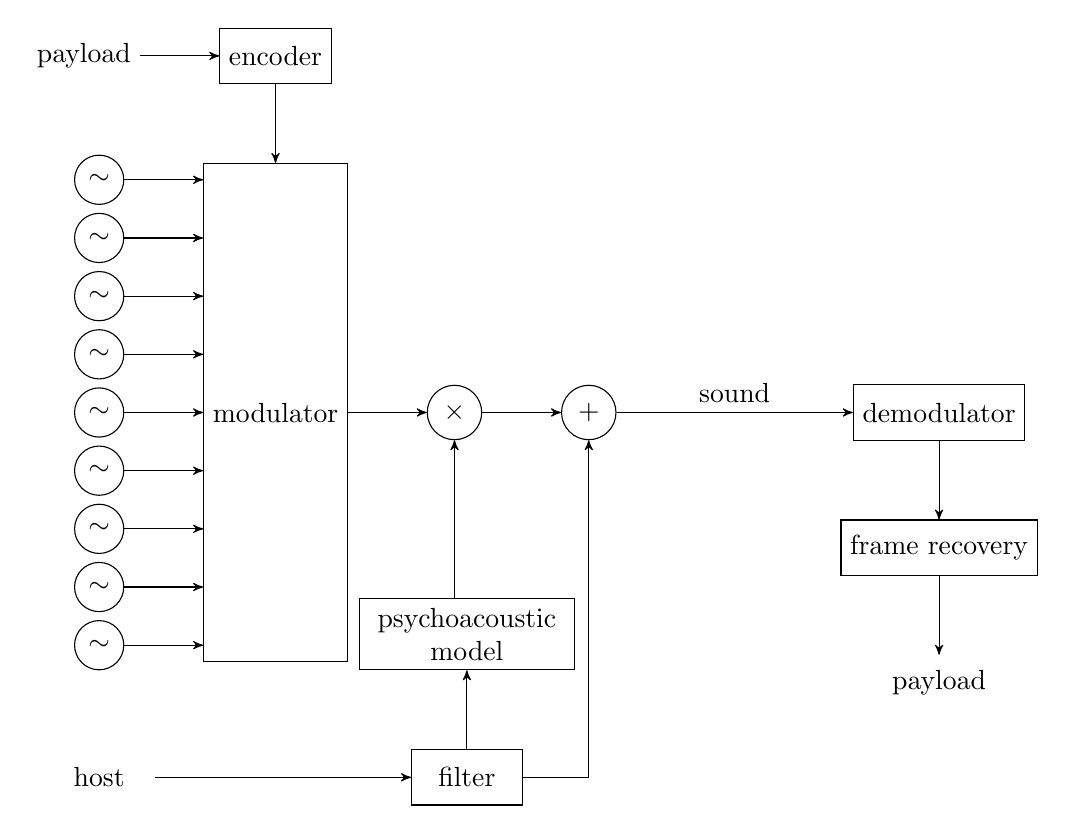
\begin{tikzpicture}[auto,node distance=1cm,>=stealth']
\tikzset{
block/.style= {draw, rectangle, minimum height=2em,minimum width=4em},
textblock/.style= {minimum height=2em,minimum width=4em},
sum/.style = {draw, circle},
oscillator/.style = {draw, circle},
input/.style  = {coordinate},
output/.style = {coordinate}
}

\node [textblock](payload) {payload};
\node [block, right = 1cm of payload](framing) {encoder};
\node [block, below = 1cm of framing, minimum height = 18em](modulator) {modulator};

\node [oscillator, left = 1cm of modulator, align = center](oscillator4) {$\sim$};
\node [oscillator, above = 0.1cm of oscillator4](oscillator3) {$\sim$};
\node [oscillator, above = 0.1cm of oscillator3](oscillator2) {$\sim$};
\node [oscillator, above = 0.1cm of oscillator2](oscillator1) {$\sim$};
\node [oscillator, above = 0.1cm of oscillator1](oscillator0) {$\sim$};
\node [oscillator, below = 0.1cm of oscillator4](oscillator5) {$\sim$};
\node [oscillator, below = 0.1cm of oscillator5](oscillator6) {$\sim$};
\node [oscillator, below = 0.1cm of oscillator6](oscillator7) {$\sim$};
\node [oscillator, below = 0.1cm of oscillator7](oscillator8) {$\sim$};

\node [textblock, below = 1cm of oscillator8](host) {host};
\node [block, right = 3.25cm of host](filter) {filter};
\node [block, above = 1cm of filter, text centered, text width = 2.5cm](psychmodel) {psychoacoustic model};
\node [sum, right = 1cm of modulator](applymodel) {$\times$};
\node [sum, right = 1cm of applymodel](sumwithhost) {$+$};
\node [block, right = 3cm of sumwithhost](demodulator) {demodulator};
\node [block, below = 1cm of demodulator](framerecovery) {frame recovery};
\node [textblock, below = 1cm of framerecovery](outputpayload) {payload};

\draw [->] (payload) -- (framing);
\draw [->] (framing) -- (modulator);
\draw [->] (oscillator0) -- (modulator.west|-oscillator0);
\draw [->] (oscillator1) -- (modulator.west|-oscillator1);
\draw [->] (oscillator2) -- (modulator.west|-oscillator2);
\draw [->] (oscillator3) -- (modulator.west|-oscillator3);
\draw [->] (oscillator4) -- (modulator.west|-oscillator4);
\draw [->] (oscillator5) -- (modulator.west|-oscillator5);
\draw [->] (oscillator6) -- (modulator.west|-oscillator6);
\draw [->] (oscillator7) -- (modulator.west|-oscillator7);
\draw [->] (oscillator8) -- (modulator.west|-oscillator8);
\draw [->] (modulator) -- (applymodel);

\draw [->] (host) -- (filter);
\draw [->] (filter) -- (psychmodel);
\draw [->] (filter) -| (sumwithhost);
\draw [->] (psychmodel.north-|applymodel) -| (applymodel);

\draw [->] (applymodel) -- (sumwithhost);

\draw [->] (sumwithhost) -- node {sound} (demodulator);

\draw [->] (demodulator) -- (framerecovery);
\draw [->] (framerecovery) -- (outputpayload);
\end{tikzpicture}
\caption{Block diagram of proposed solution}
\label{fig:solution-diagram}
\end{figure}

\section{Synthesis algorithm}

The signal synthesis algorithm has some configurable parameters:

\begin{itemize}
\item d -- duration of signal which encodes single byte (seconds)
\item fs -- sampling rate
\item sync -- synchronization signal frequency (Hertz)
\item carriers -- array of carrier signals frequencies (in Hertz)
\end{itemize}

\subsection{Data frame}

To ensure robust payload decoding in spite of transmission errors, data is encoded in frames consisting of 24 bytes:

\begin{itemize}
\item preamble -- 2 bytes
\item payload -- 16 bytes
\item error correction data -- 6 bytes
\end{itemize}

% TODO: frame visualization
A preamble is used in frame recovery algorithm~[\ref{sec:frame-recovery}] to detect frame beginning. It consists of 2 ASCII synchronous idle characters (\texttt{0x16}).
\texttt{0x} notation denotes a byte in hexadecimal format.

Error correction data is calculated from payload using Reed-Solomon~[\ref{subsec:reedsolomon}]~code.

\subsection{Carrier modulation}

Single carrier signal is a sine wave, modulated by a stream of bits using differential binary phase shift keying~[\ref{subsec:dbpsk}].

DBPSK has the advantages over other modulation methods for audio domain:~\cite{Applidium}

\begin{itemize}
\item more robust and resilient to noise than amplitude modulation
\item uses less bandwidth than frequency modulation, meaning narrower band will be removed from host signal
\item does not require reference signal in demodulator
\end{itemize}

However, sudden phase transitions required by DBPSK cause audible parasitic effects ("clicking"). To mitigate that, the parts of the signal at transition time are multiplied by cosine window.

\begin{figure}[h]
  \includegraphics[width=\linewidth]{figures/phase-transition}
  \caption{Sudden phase transition of $\pi$}
  \label{fig:phase-transition}
\end{figure}

\begin{figure}[h]
  \includegraphics[width=\linewidth]{figures/smooth-phase-transition}
  \caption{Smooth phase transition of $\pi$}
  \label{fig:smooth-phase-transition}
\end{figure}

\subsection{Byte transmission}

Total of nine sine signals are transmitted simultaneously. Eight of them each encode a single bit of a byte. The remaining signal is a synchronization signal, modulated by stream of binary ones, is used for detecting byte start\,/\,end.

% TODO: figure of synchronization signal

\subsection{Insetting in host signal}

Insetting carrier signal in host signal consists of 4 steps:

\begin{enumerate}
\item host signal is filtered with bandstop filter, removing frequencies around carrier signal
\item for each window, masking threshold for carrier signal is calculated using psychoacoustic model described in~[\ref{subsec:psychoacoustic-model}]
\item amplitude of carrier signal is multiplied by value under masking threshold
\item carrier signal is added to filtered host signal
\end{enumerate}

\section{Analysis algorithm}

Analysis algorithm shares configuration parameters with synthesis algorithm, and can further be parameterized with:

\begin{itemize}
\item ws -- window size for analysis (samples)
\end{itemize}

Each ws consecutive recorded samples are analyzed by analysis algorithm.

\subsection{Carrier demodulation}

A phase reading is obtained for each of the carrier frequencies and synchronization frequency.

For each frequency:
\begin{enumerate}
\item recorded frame is filtered with a bandpass filter centered at that frequency and multiplied by Hanning window % TODO: ref
\item phase shift relative to beginning of frame is calculated using Goertzel algorithm~[\ref{subsec:goertzel}]
\item absolute phase shift ($|\varphi|$) is obtained by calculating phase offset ($\delta\varphi$) of current frame and subtracting it from relative phase ($\varphi$).
\end{enumerate}

\begin{equation}
\delta\varphi = 2\pi(\frac{\textrm{framestart} \cdot \textrm{frequency}}{\textrm{fs}} \pmod{1.0})
\end{equation}

Where framestart is the index of the first sample of a frame in a stream of all recorded samples, and fs is sampling rate.

\begin{equation}
|\varphi| = \varphi - \delta\varphi
\end{equation}

When the synchronization signal has stable phase for the predefined number of readings (rpb -- readings per byte), it signals a byte transmission.
Phase is considered stable when standard deviation of rpb previous readings is below $\pi/5$.

\begin{equation}
\textrm{rpb} = \lfloor\frac{\textrm{fs} \cdot \textrm{d}}{\textrm{ws}}\rfloor
\end{equation}

When byte transmission occurs, previous rpb bit carrier phase readings are averaged and saved. Then the averages are compared to previous averages and if difference of $\pi$ is detected, a binary 1 is decoded. Otherwise, binary 0 is decoded.

Eight bits decoded from carrier signals are then combined to form a single byte, which gets forwarded to frame recovery algorithm.

\subsection{Frame recovery}
\label{sec:frame-recovery}

A simple frame recovery algorithm scans the byte stream for preamble bytes.
However, since transmission error might have occurred and preamble might be scrambled, the algorithm has to evaluate each consecutive pair of bytes as a candidate for being a preamble.

It assigns a score for each position in bit stream, calculated as follows:

\begin{equation}
\textrm{score} = 1 - \frac{\textrm{pop(bit0 xor \texttt{0x16})} + \textrm{pop(bit1 xor \texttt{0x16})}}{16}
\end{equation}

(where pop is a function returning number of set bits in a byte).

Score of 1 means exact preamble is detected. However, if no preamble position is found, the algorithm waits for next 24 bytes to calculate the score of a position a frame size bytes ahead. If that score is large enough, previous position is selected as frame beginning.

Once beginning of frame is identified and all frame bytes are received, the algorithm extracts payload data, tries to apply Reed-Solomon error correction to correct any transmission errors, and returns decoded part of payload data.

\chapter{Implementation}

\section{Programming environment}

The solution is implemented in python programming language. Python was chosen because of authors' previous experience with it, ease of programming and prototyping, and availability of digital signal processing and utility libraries.

Following python libraries are used:

\begin{itemize}
  \item numpy -- math and array manipulation library
  \item scipy -- digital signal processing algorithms
  \item matplotlib -- graphing
  \item reedsolo -- implementation of Reed-Solomon code
  \item pyaudio -- playing and recording sound
\end{itemize}

Main result of work is a python library, with few dependencies, which is portable and can be used in many applications (some are discussed in the~\nameref{chap:summary} chapter)

\section{Outline of implementation}

The library consists of core emitter and receiver modules, as well as several other additional modules.

Emitter and receiver are meant to be used separately each for its own application, and are orthogonal
to sound playing/recording concerns. This makes them portable across platforms that support python programming language.
Only configuration parameters (synchronization and carrier frequency values) must be shared between receiver and emitter.

\clearpage

\section{Emitter}

Emitter class implements synthesis algorithm described in chapter \ref{chap:solution}. With emitter object, an application can obtain samples of host sound with payload data hidden in it.

Public methods:

\begin{itemize}
\item \verb|Emitter(host, sample_rate, sync_frequency, carrier_frequencies, payload)|

  Constructor

  Arguments:
  \begin{itemize}
  \item \verb|host| -- sampled host signal (\verb|numpy.float32| array)
  \item \verb|sample_rate| -- sampling rate of host signal (\verb|float|)
  \item \verb|sync_frequency| -- synchronization frequency in Hertz (\verb|float|)
  \item \verb|carrier_frequencies| -- list of carrier frequencies in Hertz (list of eight \verb|float|)
  \item \verb|payload| -- bytes to be transmitted (list of \verb|int|)
  \end{itemize}

  Return value: \verb|emitter|
  \begin{itemize}
  \item \verb|emitter| -- instance of Emitter
  \end{itemize}

\item \verb|outstream(buf)|

  When this method is called, emitter will start putting chunks of synthesized samples on the \verb|buf| queue. The caller can then forward these samples to hardware loudspeakers.

  Putting \verb|False| boolean on the queue signals end of synthesized signal.

  Arguments:
  \begin{itemize}
  \item \verb|buf| -- FIFO queue for putting chunks of synthesized sound on (python \verb|Queue|)
  \end{itemize}

  Return value: \verb|buf|
  \begin{itemize}
  \item \verb|buf| -- the same as first argument.
  \end{itemize}

\end{itemize}

See Figure \ref{fig:emitter-application} for example usage of emitter in an application.

\begin{figure}[h]
\centering
\inputminted[linenos]{python}{listings/emitter_example.py}
\caption{Example usage of emitter in an application}
\label{fig:emitter-application}
\end{figure}

\clearpage

\section{Receiver}

Receiver class implements analysis algorithm described in chapter \ref{chap:solution}. With receiver object, an application can decode payload data from recorded sound samples.

Public methods:

\begin{itemize}
\item \verb|Receiver(instream, sample_rate, sync_frequency, carrier_frequencies)|

  Constructor

  Arguments:
  \begin{itemize}
  \item \verb|instream| -- queue for incoming recorded samples (python \verb|Queue|)
  \item \verb|sample_rate| -- sampling rate (\verb|float|)
  \item \verb|sync_frequency| -- synchronization frequency in Hertz (\verb|float|)
  \item \verb|carrier_frequencies| -- list of carrier frequencies in Hertz (list of eight \verb|float|)
  \end{itemize}

  Return value: \verb|receiver|
  \begin{itemize}
  \item \verb|receiver| -- instance of Receiver
  \end{itemize}

\item \verb|payload_stream(outstream)|

  After calling this method, decoded bytes of data will be put on the queue.

  Putting \verb|False| boolean on the queue means end of decoded data.

  Arguments:
  \begin{itemize}
  \item \verb|outstream| -- FIFO queue for putting decoded bytes on (python \verb|Queue|)
  \end{itemize}

  Return value: \verb|outstream|
  \begin{itemize}
  \item \verb|outstream| -- the same as first argument.
  \end{itemize}

\end{itemize}

See Figure~\ref{fig:receiver-application} for example usage of receiver in an application.

\clearpage

\begin{figure}[h]
\centering
\inputminted[linenos]{python}{listings/receiver_example.py}
\caption{Example usage of receiver in an application}
\label{fig:receiver-application}
\end{figure}

\section{Other modules}

\subsection{Encoder}

This sub-module implements \emph{encoding} block from Figure~\ref{fig:solution-diagram}.

Encoder is responsible for splitting the payload data into frames (adding preamble, calculating Reed-Solomon error correction) and outputting stream of bits ready for transmission. In case payload data cannot be split evenly into frames, it is zero-padded to required length.

Public methods:

\begin{itemize}
\item \verb|Encoder(payload)|

  Constructor

  Arguments:
  \begin{itemize}
  \item \verb|payload| -- data to be encoded (list of \verb|int|)
  \end{itemize}

  Return value: \verb|encoder|
  \begin{itemize}
  \item \verb|encoder| -- instance of Encoder
  \end{itemize}

\item \verb|encode()|

  Encodes payload into stream of bytes ready for transmission.

  Arguments: none

  Return value: \verb|out|
  \begin{itemize}
  \item \verb|out| -- encoded bytes (list of \verb|int|)
  \end{itemize}

\end{itemize}

See Figure~\ref{fig:encoder-example} for example usage in code.

\begin{figure}[p]
\centering
\inputminted[linenos]{python}{listings/encoder_example.py}
\caption{Usage of encoder}
\label{fig:encoder-example}
\end{figure}

\subsection{Decoder}

This sub-module implements \emph{frame recovery} block from Figure~\ref{fig:solution-diagram}.

Decoder is a stateful object responsible for scanning incoming stream of data, extracting correct frames (see~\ref{sec:frame-recovery}), applying error correction code and outputting decoded payload data.

Public methods:

\begin{itemize}
\item \verb|Decoder()|

  Constructor

  Arguments: none

  Return value: \verb|decoder|
  \begin{itemize}
  \item \verb|decoder| -- instance of Decoder
  \end{itemize}

\item \verb|add(byte)|

  Registers incoming byte in decoder

  Arguments:
  \begin{itemize}
  \item \verb|byte| -- incoming byte (\verb|int|)
  \end{itemize}

  Return value: none

\item \verb|can_decode()|

  Arguments: none

  Return value: \verb|can|
  \begin{itemize}
  \item \verb|can| -- \verb|True| if decoder has enough bytes to decode a frame. Otherwise \verb|False|
  \end{itemize}

\item \verb|decode()|

  Decodes payload data from incoming bytes

  Arguments: none

  Return value: \verb|(bytes, frame_count)|
  \begin{itemize}
  \item \verb|bytes| -- list of decoded payload bytes (list of \verb|int|)
  \item \verb|frame_count| -- how many frames were decoded (\verb|int|)
  \end{itemize}
\end{itemize}

See Figure~\ref{fig:decoder-example} for example usage in code.

\begin{figure}[p]
\centering
\inputminted[linenos]{python}{listings/decoder_example.py}
\caption{Usage of decoder}
\label{fig:decoder-example}
\end{figure}

\subsection{Goertzel}

This sub-module implements Goertzel algorithm generalized to non-integer multiple of fundamental frequency, as described in~\cite{PS12}.

Public methods:
\begin{itemize}
\item \verb|goertzel(x, k)|

  Calculates spectral component \verb|k| of signal \verb|x|.

  Frequency of component can be calculated as \verb|k * fs / N| where \verb|fs| is sampling rate, and \verb|N| is length of \verb|x|.

  Arguments:
  \begin{itemize}
  \item \verb|x| -- signal (list of \verb|float|/\verb|complex| numbers)
  \item \verb|k| -- spectral component index (\verb|float|)
  \end{itemize}

  Return value: \verb|y|
  \begin{itemize}
  \item \verb|y| -- spectral component (\verb|complex| number)
  \end{itemize}
\end{itemize}

\subsection{Psychoacoustic analyzer}

This sub-module implements \emph{psychoacoustic model} described in~\ref{subsec:psychoacoustic-model}.

Public methods:

\begin{itemize}
\item \verb|masking_threshold(x, f, fs)|

  For given chunk of sound and frequency, this method calculates masking threshold under which components with
  given frequency are inaudible.

  Arguments:
  \begin{itemize}
  \item \verb|x| -- signal to calculate masking threshold for (list of \verb|float|)
  \item \verb|f| -- frequency to calculate masking threshold for (\verb|float|)
  \item \verb|fs| -- sampling rate (\verb|float|)
  \end{itemize}

  Return value: \verb|threshold|
  \begin{itemize}
  \item \verb|threshold| -- masking threshold for frequency \verb|f| in sound \verb|x| (\verb|float|)
  \end{itemize}
\end{itemize}

\subsection{Graphing utilities}

The system includes graphing sub-module that can optionally plug into receiver module and plot phase readings, bit synchronization, and frame synchronization moments (see Figure~[\ref{fig:graph-utility}]).
This module has capability to plot values after all payload data was received as well as in real time.

\begin{figure}[p]
  \centering
  \includegraphics[width=\linewidth]{figures/graph_example}
  \caption{An example screen of graph utility}
  \label{fig:graph-utility}
\end{figure}

\chapter{Tests}
\label{chap:tests}

\section{Tests outline}

Two kinds of tests examining different sides of solution are performed:
\begin{itemize}
  \item performance tests -- laboratory tests examining designed solution's performance in various conditions
  \item psychoacoustic test -- experiment examining audibility of signal hidden by presented solution
\end{itemize}

\noindent In every type of test, synthesis\,/\,analysis algorithms are parameterized with following values:

\begin{itemize}
  \item byte duration = 200\,ms
  \item carrier signal band = 8000--8800\,\mbox{Hz}
\end{itemize}

With this setup, the solution achieves effective data bandwidth of 26.66\,\mbox{bps} (bits per second).

Unfortunately tests are not performed on mobile platform because of longer time required for implementation. All performance tests 
are conducted in acoustic laboratory using stationary devices.

\section{Performance tests}
\subsection{Overview}
The purpose of performance tests is to examine the possibilities of implemented solution. Information about algorithm effectiveness is expected as an procedure output.
Performance tests are conducted in a laboratory environment to enable environment manipulation.
To get most informative output data and effective testing environment, following features are required:
\begin{itemize}
  \item value-neutrality -- any kind of unwanted environmental noise is eliminated
  \item versatility -- various environment conditions are simulated
  \item repeatability -- tests are easy to conduct and repeat many times in the same form.
\end{itemize}

To fulfill the requirements, anechoic chamber and professional recording\,/\,playback facilities are employed.
See Figure \ref{fig:test-environment} for block diagram of test environment setup.

\clearpage

\subsection{Environment setup}
\begin{figure}[h]
  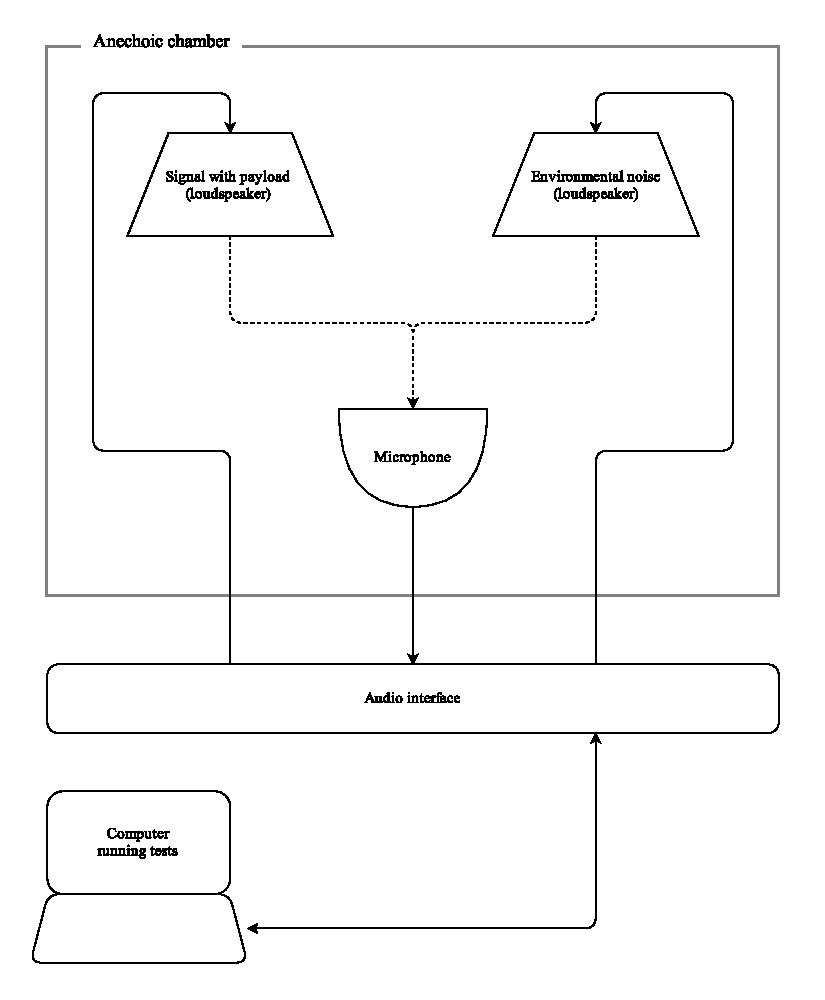
\includegraphics[width=\linewidth]{figures/experiments/environment}
  \caption{Test environment diagram}
  \label{fig:test-environment}
\end{figure}
Two loudspeakers are directed to microphone in monophonic mode. Microphone output is connected to audio interface input. Loudspeakers are connected to separate
interface outputs. Computer plays encoded signal on one speaker and environmental noise on the other one. At the same time, audio signal is
recorded using the microphone. Recorded samples are then analyzed using developed solution. The decoded payload is compared to original and Bit Error Rate (BER) is computed.

\clearpage

Following equipment is used to realize described solution:
\begin{itemize}
\item 2 $\times$ Tannoy 800A Active monitor loudspeakers
\item Shure VP88 MS-stereo-condenser microphone
\item Focusrite Scarlett 18i20 USB Audio interface
\item MacBook Air with OS X Yosemite (10.9)
\end{itemize}

\subsection{Implementation}

Test software is implemented in python programming language, like the algorithm library. The language was chosen to stay consistent across entire solution.
It is also easy to utilize encoding\,/\,decoding library written in the same language.
The \verb|Experiment| class is responsible for conducting performance tests.

Public methods:
\begin{itemize}
  \item \verb|Experiment(host, noise, host_db, noise_db, payload)|
    Constructor

    Arguments:
    \begin{itemize}
      \item \verb|host|\quad host signal file path (\verb|string|)
      \item \verb|noise|\quad noise signal file path (\verb|string|)
      \item \verb|host_db|\quad amplitude of host signal in \mbox{dB} (\verb|float|)
      \item \verb|noise_db|\quad amplitude of noise signal in \mbox{dB} (\verb|float|)
      \item \verb|payload|\quad bytes to be transmitted (list of \verb|int|)
    \end{itemize}

  \item \verb|run()|

    When this method is called, experiment procedure starts. After conducted experiment, all parameters with decoded payload are appended in python format to \verb|experiment_output.txt| file.

    Return value: \verb|decoded_payload|
    \begin{itemize}
    \item \verb|decoded_payload| – payload decoded from recorded sample (array of \verb|int|)
    \end{itemize}

  \item \verb|BER(correct, computed)|

    Static class method.
    It reckons bit error rate for decoded payload data.

    Arguments:
    \begin{itemize}
      \item \verb|correct| -- original payload (array of \verb|int|)
      \item \verb|computed| -- decoded payload (array of \verb|int|)
    \end{itemize}

    Return value: \verb|bit_error_rate|
    \begin{itemize}
      \item \verb|bit_error_rate| -- reckoned bit error rate
    \end{itemize}

\end{itemize}

See Figure \ref{fig:experiment-application} for example usage of \verb|Experiment| class in an application.
\begin{figure}[h]
  \centering
  \inputminted[linenos]{python}{listings/experiment_example.py}
  \caption{Example usage of experiment class in an application}
  \label{fig:experiment-application}
\end{figure}

\subsection{Sound samples}
\label{subsec:sound-samples}
Two types of sound samples are needed to conduct performance tests:
\begin{itemize}
  \item host samples -- three sampled pieces of music to host encoded payload
  \item noise samples -- four various environmental noises
\end{itemize}
All audio samples used in tests are 24-bit monophonic WAV files. All spectrum charts have red-marked region in frequency range
used by presented solution. In case of noise signals -- they should disturb decoding process as much as there is power in this range.

\subsubsection{Noise samples}
All environmental noise is recorded especially for the purpose of the project. From many recorded sounds, only
three probes were selected. The selection is based on spectral analysis. Only sound samples containing much power in carrier signal
band are used.
Following four pieces were selected:
\begin{itemize}
  \item \verb|ambulance.wav| -- ambulance emergency signal (See: Figure \ref{fig:ambulance-analysis})
  \item \verb|bottle-scratch.wav| -- sound of scraping glass bottles (See: Figure \ref{fig:bottle-scratch-analysis})
  \item \verb|crowd.wav| -- speaking crowd (See: Figure \ref{fig:crowd-analysis})
  \item \verb|keys.wav| -- clanking keys (See: Figure \ref{fig:keys-analysis})
\end{itemize}


\noindent To record these sounds following equipment has been used:
\begin{itemize}
  \item Tascam DR-40 Linear PCM hand-recorder
  \item Shure VP88 MS-stereo-condenser microphone with foam windscreen
\end{itemize}

\clearpage

Noise samples spectral charts:

\begin{figure}[!hb]
\centering
\begin{minipage}[b]{0.45\textwidth}
  \includegraphics[width=\textwidth]{figures/experiments/spectrum_ambulance.png}
  \captionof{figure}{ambulance.wav spectrum}
  \label{fig:ambulance-analysis}
\end{minipage}\hfill
\begin{minipage}[b]{0.45\linewidth}
  \includegraphics[width=\textwidth]{figures/experiments/spectrum_bottle-scratch.png}
  \captionof{figure}{bottle-scratch.wav spectrum}
  \label{fig:bottle-scratch-analysis}
\end{minipage}
\end{figure}
\begin{figure}[!hb]
\begin{minipage}[b]{0.45\textwidth}
  \includegraphics[width=\linewidth]{figures/experiments/spectrum_crowd.png}
  \captionof{figure}{crowd.wav spectrum}
  \label{fig:crowd-analysis}
\end{minipage}\hfill
\begin{minipage}[b]{0.45\textwidth}
  \includegraphics[width=\linewidth]{figures/experiments/spectrum_keys.png}
  \captionof{figure}{keys.wav spectrum}
  \label{fig:keys-analysis}
\end{minipage}
\end{figure}

\subsubsection{Host samples}
An important requirement is to make the carrier signal inaudible. In the experiments, only musical pieces
are used as a host signals, as music contains various partials which can be used for masking. Musical genres diversity is guaranteed.
Three host signals are selected for testing purposes:
\begin{itemize}
  \item \verb|bach.wav| -- (classical) fragment of "Gloria in excelisis deo" composed by J.S. Bach (See: Figure \ref{fig:bach-analysis})
  \item \verb|rockvocals.wav| -- (rock) fragment of "Can't stop" by Red Hot Chilli Peppers(See: Figure \ref{fig:rockvocals-analysis})
  \item \verb|skalpel.wav| -- (hip-hop) fragment of "Adventures in space" by Skalpel (See: Figure \ref{fig:skalpel-analysis})
\end{itemize}

\clearpage
\noindent Host samples spectral charts:

\begin{figure}[!hb]
\begin{minipage}[b]{0.45\textwidth}
  \includegraphics[width=\linewidth]{figures/experiments/spectrum_bach.png}
  \captionof{figure}{bach.wav spectrum}
  \label{fig:bach-analysis}
\end{minipage}\hfill
\begin{minipage}[b]{0.45\textwidth}
  \includegraphics[width=\linewidth]{figures/experiments/spectrum_rockvocals.png}
  \captionof{figure}{rockvocals.wav spectrum}
  \label{fig:rockvocals-analysis}
\end{minipage}
\end{figure}
\begin{figure}[!hb]
\begin{minipage}[b]{0.45\textwidth}
  \includegraphics[width=\linewidth]{figures/experiments/spectrum_skalpel.png}
  \captionof{figure}{skalpel.wav spectrum}
  \label{fig:skalpel-analysis}
\end{minipage}
\end{figure}

\clearpage

\subsubsection{Sound sample with hidden information}
After insetting encoded payload information into the host signal, spectrum changes significantly.
The amount of influence that can be seen on spectrum depends on psychoacoustic model adjustment of amplitude, which in turn depends on number and power of maskers around chosen frequency band.

\newsubfloat{figure}

\begin{figure}[!hb]
  \begin{minipage}[b]{0.45\textwidth}
    \includegraphics[width=\linewidth]{figures/experiments/spectrum_bach}
    \subcaption{Original signal}
  \end{minipage}\hfill
  \begin{minipage}[b]{0.45\textwidth}
    \includegraphics[width=\linewidth]{figures/experiments/spectrum_bach_altered}
    \subcaption{Signal with an inset information}
  \end{minipage}
  \caption{Difference between signal spectrum}
\end{figure}

\clearpage

\subsection{Test results}
Tests are performed according to following rules:
\begin{enumerate}
  \item for each host signal take every noise signal
  \item for each \verb|(host, noise)| pair take every amplitude from \verb|[-30,-20,-15,-10,-5,0]|\,\mbox{dB}
  \item perform test for each \verb|(host, noise, amplitude)| tuple
\end{enumerate}
All tests are performed three times and average from their BER is reckoned. In most cases BER is equal to 0, however there
are two particular cases worth explaining.

\subsubsection{Frame detection failure}
\label{subsub:frame-detection}
This situation causes very high BER value. It happens when the system is unable to recover frame beginning and it waits till next frame.
In effect it omits single bit of data. It causes a shift of entire decoded data by 1 byte to the left. It is dangerous situation, because decoded data
can be completely useless even if this type of failure does not seem to be a big mistake.
\begin{figure}[hb]
\begin{minipage}[b]{0.45\textwidth}
  \includegraphics[width=\linewidth]{figures/experiments/BER_bach_crowd}
\end{minipage}\hfill
\begin{minipage}[b]{0.45\textwidth}
  \includegraphics[width=\linewidth]{figures/experiments/BER_bach_keys}
\end{minipage}\hfill
\label{fig:frame-failure}
\caption{Frame detection failure}
\end{figure}

\clearpage

\subsubsection{Single bit mis-decoding}
It is the case when the system decodes single bit improperly. It raises the BER index, but not as much as in the frame detection failure case.
In this situation the recovered payload is more likely to be usable, because it is not shifted.
\begin{figure}[!hb]
\begin{minipage}[b]{0.45\textwidth}
  \includegraphics[width=\linewidth]{figures/experiments/BER_rockvocals_crowd}
\end{minipage}\hfill
\begin{minipage}[b]{0.45\textwidth}
  \includegraphics[width=\linewidth]{figures/experiments/BER_rockvocals_bottle-scratch}
\end{minipage}
\end{figure}
\begin{figure}[!hb]
\begin{minipage}[b]{0.45\textwidth}
  \includegraphics[width=\linewidth]{figures/experiments/BER_skalpel_keys}
\end{minipage}\hfill
\begin{minipage}[b]{0.45\textwidth}
  \includegraphics[width=\linewidth]{figures/experiments/BER_skalpel_bottle-scratch}
\end{minipage}
\label{fig:mis-decoding}
\caption{Single bit mis-decoding}
\end{figure}
\begin{figure}[!hb]
\begin{minipage}[b]{0.45\textwidth}
  \includegraphics[width=\linewidth]{figures/experiments/BER_bach_bottle-scratch}
\end{minipage}\hfill
\end{figure}

\clearpage

\section{Psychoacoustic test}
\label{sec:psychoacoustic-test}

\subsection{Overview}
A purpose of this type of test is to examine how human auditory system (See: \ref{subsec:human-auditory}) reacts to data hidden
in host audio signal. The goal of presented solution is to make hidden carrier signal inaudible for humans. The experiment is conducted
on a sample of 20 people.

\subsection{Experiment process}
\begin{enumerate}
  \item two versions of every examined sound sample are prepared. The first one with original sound and the second one with hidden carrier signal
  \item a test form is provided to each participant. The form contains three rows (sample names) and two columns (sample versions)
  \item for each examined sound sample pair a coin toss is performed. Toss result determines sound sample playback order
  \item participant listens to two sound samples
  \item participant puts a mark in column corresponding to the version they think is deformed by the hidden carrier
  \item filled forms are compared to the reference form containing only sound samples correctly identified as containing payload
\end{enumerate}

\subsection{Test results}
Obtained results indicate significant problems with differentiating original sound from sound with hidden data. It means signal
is well-hidden and inaudible (in most cases) for humans.

\begin{figure}[!hb]
  \centering
  \includegraphics[width=0.6\linewidth]{figures/experiments/psychoacoustic}
  \label{fig:psychoacoustic-results}
  \caption{Results of psychoacoustic test}
\end{figure}

As it can be seen on above chart, the most accurate identifications belong to \verb|bach.wav| sound sample -- less opportunity for masking causes easier recognition of signal deformation.
See Figure \ref{fig:bach-analysis} for \verb|bach.wav| spectrum.

\section{Conclusions}
The performed tests prove the requirements are met:
\begin{itemize}
  \item hidden signal is inaudible for humans
  \item encoded payload is recoverable from the recorded sound sample.
\end{itemize}

However, designed solution is not perfect. Tests created a possibility to notice major issues like frame detection failure
cases (see: \ref{subsub:frame-detection}). Although it can be a significant trammel in using developed library, solution
still handles really difficult environment conditions. All failure recovery tries are related to noise source set to maximum 
tested amplitude. In all cases when noise signal amplitude is lower than encrypted host amplitude, receiver decodes data correctly.
The system needs only little enhancement to become profoundly usable python library for hiding data in audio signals.

\chapter{Summary}
\label{chap:summary}

The thesis presents a solution for insetting and recovery of data in sound in imperceptible way, as well as
implementation of the solution.

The solution is shown to allow a robust transmission in presence of interference (in laboratory conditions) and to be
imperceptible to human listeners (See \ref{sec:psychoacoustic-test}).

\section{Possible applications}

The python library developed as a part of this thesis can be utilized on many platforms that support python programming language.

Example applications might include:

\begin{enumerate}
\item In marketing -- embedding data in advertisements.

Data like product details or promotional coupons could be hidden in advertisement music. Consumers would be able to
extract and use this data using smartphone application.

\item In broadcasting -- embedding meta-data in music.

Meta-data like artist name, song title or even song lyrics could be hidden in music broadcasted on live events.
Listeners would be able to access it using mobile application.

\item In digital rights management -- a simple watermark.

Watermark data could be hidden in music or film score to detect copyright infringement. The disadvantage of presented
solution is ease of watermark removal.
\end{enumerate}

\section{Possible improvements}

\begin{itemize}
\item Increase data bandwidth

Transmission bandwidth achieved in the implemented solution might limit the number of applications.
Bandwidth could be increased by decreasing single byte transmission duration and using phase recovery method
less susceptible to noise.

\item Improve frame recovery algorithm

Implemented frame recovery algorithm is shown to fail to correctly detect a frame in some conditions (see~\ref{subsub:frame-detection}).
This could be improved by using longer preamble or another method for synchronizing frames.

\item Evaluation in real-life conditions

The tests in Chapter \ref{chap:tests} are performed in laboratory conditions. Additional tests should be
performed to evaluate the system's performance in presence of natural phenomena (like echoes) and using commodity hardware.

\item Advanced psychoacoustic model

Another psychoacoustic model might be implemented, exploiting additional properties of human auditory system, like
temporal masking~(\ref{itm:masking-effects}).

\item Implementation of mobile application

A showcase application for easy broadcasting and receiving of data, running on any of major mobile operating systems.
\end{itemize}

\section{Acknowledgments}

Authors would like to thank prof.~dr. hab.~inż~Adam Dąbrowski and dr. Szymon Drgas for support in designing a solution,
and dr.~inż. Andrzej Meyer for help with laboratory and audio equipment.


% All appendices and extra material, if you have any.
\cleardoublepage\appendix%

\listoffigures

% Bibliography (books, articles) starts here.
\addtocontents{toc}{\protect\enlargethispage{\baselineskip}} % HACK: prevent table of contents from spilling to second page
\bibliographystyle{alpha}{\raggedright\sloppy\small\bibliography{bibliography}}

% Colophon is a place where you should let others know about copyrights etc.
\ppcolophon

\end{document}
